%!TEX root=../robocert.tex
\begin{figure}
	\centering
	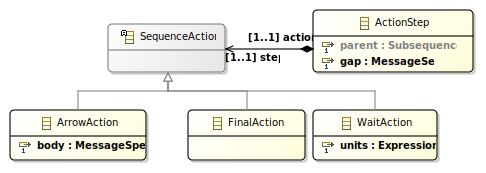
\includegraphics[width=0.7\textwidth]{diagrams/Actions}
	\caption{Class diagram for the part of the \langname{} metamodel dealing with actions.}
	\label{fig:metamodel-actions}
\end{figure}

\Cref{fig:metamodel-actions} depicts the part of the metamodel concerning
sequence actions.

A \msequenceaction{} is a construct in a \msubsequence{} that, informally,
represents an activity on the sequence diagram that takes time to perform.
(Formally speaking, most \msequenceaction s are instantaneous but
allow time to pass immediately beforehand.)

There are currently three types of action: arrow, wait, and
final actions.

\subsection{\marrowaction}

An \marrowaction\footnote{The name signifies both that the actions resemble
PSC \emph{arrowMSG} specifications, and also that they correspond to arrows in
the graphical syntax.} explicitly specifies a communication between \mactor s.
Each \marrowaction{} wraps one
\marrowmessagespec{} (\cref{sec:metamodel-messages})
containing the specification proper.
\todo{Eventually these will bind arguments.}

\begin{figure}[h!]
\begin{subfigure}[t]{\egtextwidth}
\begin{lstlisting}[style=Example]
->op O1()
\end{lstlisting}
\end{subfigure}
\hfill
\begin{subfigure}[t]{\eggraphicalwidth}
\gsecaption
\centering
\begin{tikzpicture}
\matrix[diagram]{
    \node[rcmodule](mstart) {\egtarget}; & \node[world](wstart) {\egworld}; \\
	\coordinate(mo); & \coordinate(wo); \\
	\coordinate(mend); & \coordinate(wend); \\
};
\draw[lifeline] (mstart) -- (mo) -- (mend);
\draw[lifeline] (wstart) -- (wo) -- (wend);
\draw (mo) edge[oarrow, "O1()"] (wo);
\end{tikzpicture}
\end{subfigure}

\end{figure}

\subsection{\mwaitaction}

A \mwaitaction{} represents a pause for a specific number of time
units.

The effect of a \msequencegap{} on a \mwaitaction{} is perhaps subtle:
the gap remains active until the wait has concluded.  For instance,
a wait for \(3\) time units allows any communication on the gap to
occur for \(3\) time units.

\todo{nondeterministic wait}

\begin{figure}[h!]
\begin{subfigure}[t]{\egtextwidth}
\begin{lstlisting}[style=Example]
wait for 3 units
\end{lstlisting}
\end{subfigure}
\hfill
\begin{subfigure}[t]{\eggraphicalwidth}
\gsecaption
\centering
\begin{tikzpicture}
\matrix[diagram]{
    \node[rcmodule](mstart) {\egtarget}; & \node[world](wstart) {\egworld}; \\
	\coordinate(mw); & \coordinate(ww); \\
	\coordinate(mend); & \coordinate(wend); \\
};
\draw[lifeline] (mstart) -- (mw) -- (mend);
\draw[lifeline] (wstart) -- (ww) -- (wend);
\gwait{mw}{ww}{3}
\end{tikzpicture}
\end{subfigure}

\end{figure}

\subsection{\mfinalaction}

A \mfinalaction{} captures the eventual successful termination of a
sequence diagram.  A diagram with a \mfinalaction{} specifies a
complete sequence of behaviour from the \mtarget{} initialising to the
\mtarget{} terminating.  Conversely, sequence diagrams without
\mfinalaction s capture partial specifications of behaviour, or the
behaviour of \mtarget s that do not terminate.

Note that the final \msequencegap{} before a \mfinalaction{} captures
any permitted communications after the behaviour explicitly specified by the
diagram has occurred.

\begin{figure}[h!]

\begin{subfigure}[t]{\egtextwidth}
\begin{lstlisting}[style=Example]
end
\end{lstlisting}
\end{subfigure}
\hfill
\begin{subfigure}[t]{\eggraphicalwidth}
\gsecaption
\centering
\begin{tikzpicture}
\matrix[diagram]{
	\node[rcmodule](mstart) {\egtarget}; & \node[world](wstart) {\egworld}; \\
	\coordinate(mend); & \coordinate(wend); \\
};
\draw[lifeline] (mstart) -- (mend);
\draw[lifeline] (wstart) -- (wend);
\gfinal{mend}{wend}
\end{tikzpicture}
\end{subfigure}

\end{figure}

%%% Local Variables:
%%% mode: latex
%%% TeX-master: "../robocert"
%%% End:
